

\chapter{Les réseaux à convolutions}


\section{Présentation générale}

\subsection{Introduction}
L'architecture d'un multiperceptron se prête bien à des applications simplistes comme de la reconnaissance de chiffre. Cependant, dès que la complexité des données augmente ne serait-ce que légèrement, le MLP devient inefficace en un temps raisonnable pour pouvoir reconnaitre des objets. Heureusement, il existe une structure bien plus efficace qui est parfaitement adaptée à la reconnaissance d'image : le \textbf{CNN (convolutional neural network)}. L'idée de cette architecture a été introduite en 1980 \cite{fukushima_neocognitron_1980} et a ensuite été développée par Yann LeCun \cite{lecun_gradient-based_1998} pour donner naissance plus récemment à des réseaux comme AlexNet \cite{krizhevsky_imagenet_2012} ou Inception \cite{szegedy_going_2014}. Les couches à convolutions sont maintenant indispensables à la plupart des réseaux traitant des informations structurées compositionnelles.

\subsection{Structure d'un CNN}
La structure d'un CNN se rapproche de celle d'un multiperceptron dans la mesure où celui-ci est aussi organisé sous forme de couches comme le montre la figure \ref{structure_1}. Cependant, certaines couches, nommées couches de convolution, ont un fonctionnement radicalement différent de celui d'une couche dense. \\

\begin{figure}[!h]
\centering
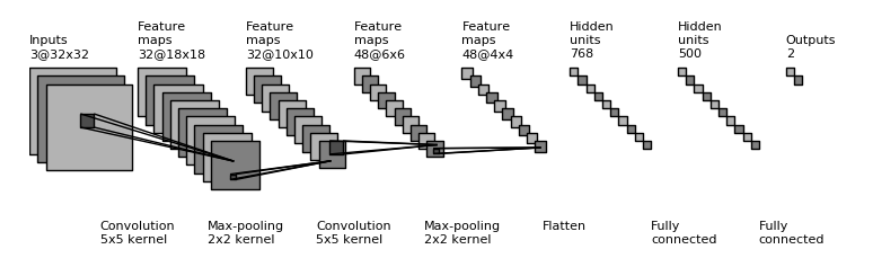
\includegraphics[width=200pt]{images/cnn/structure_CNN.png} 
\caption{Structure simplifiée d'un CNN. L'image est tirée de \cite{jefkine_backpropagation_2016} }
\label{structure_1}
\end{figure}

Ainsi, l'image en entrée est d'abord traitée par une succession de \textbf{couches de convolutions} suivies d'une \textbf{couche de pooling}. Ensuite ce processus se répète un certain nombre de fois et finalement le résultat passe par une ou plusieurs couches denses qui jouent le rôle d'un classifieur classique.

\subsection{Principe général}
Le principe directeur se cachant derrière les couches de convolution se base sur le fonctionnement même de notre vision : on dispose d'un noyau (\textit{kernel}) capable de reconnaître un motif en particulier. Il suffit alors de balayer l'image pixel par pixel (le balayage sera expliqué plus en détails ultérieurement) pour savoir où se trouvent précisément certains motifs sur l'image. En répétant ce procédé avec un grand nombre de noyaux différents, nous sommes capables de pouvoir identifier la présence ou non de certains motifs caractéristiques de l'objet à reconnaître. \\
Nous disposons ainsi d'une "carte" des différents motifs. Il nous est possible de la réduire en taille (étape de \textit{pooling}) pour réduire le nombre de calculs à effectuer. 
Le processus se répète un certain nombre de fois jusqu'à ce que l'on considère que les données soient suffisamment bien réduites pour qu'un MLP puisse s'en charger. 

\section{Formalisation d'un CNN}

\subsection{Le produit de convolution : un outil indispensable}

Le coeur de l'efficacité d'un CNN repose sur le produit de convolution. On assimile l'image à une matrice notée $I$ (nous la supposons pour l'instant en niveau de gris, de telle sorte que la matrice est en 2D mais la généralisation en 3D se fait aisément). De même, le noyau sera noté sous la forme d'une matrice $K$.
L'opération de convolution s'écrit alors : \\

$\forall (x,y) \in [0,W_I] \times [0,H_I] \, entiers \, $,  $(N \otimes I)_{x,y} = \sum_{i=0}^{W_K} \sum_{j=0}^{H_K} K_{i,j} \times I_{x-i,y-j}$ \\
\\
Où l'on a posé $W_I,H_I$ la taille de l'image et $W_K,H_K$ la taille du noyau. \\
\\
La figure \ref{chien_prairie} donne quelques exemples de l'effet du produit de convolution avec plusieurs noyaux.

\begin{figure}[!h]
\centering
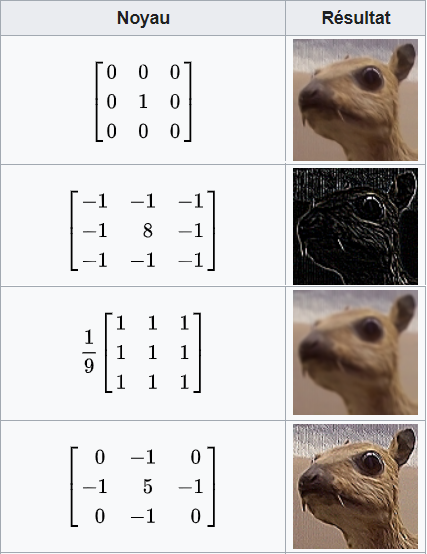
\includegraphics[width=100pt]{images/cnn/chien_prairie.png} 
\caption{Effets de la convolution avec quelques noyaux. L'image provient de Wikipedia.}
\label{chien_prairie}
\end{figure}

Ainsi, cette opération nous permet de mettre en évidence des motifs élémentaires en activant la case correspondante si le motif est présent au niveau de celle-ci.

\subsection{Le balayage de l'image : une histoire de Padding et de Stride}

Pour pouvoir évaluer toute l'image, il va falloir la balayer avec le noyau. De manière assez logique, on commence par se placer sur le coin supérieur gauche de l'image, puis on effectue un produit de convolution. Ensuite, il suffit de faire glisser latéralement le noyau d'un pixel et de répéter l'opération. Une fois au bout de la ligne, on descend d'un pixel et on repart à gauche. La figure \ref{convolution} donne un exemple de balayage d'un noyau sur une image.

\begin{figure}[!h]
\centering
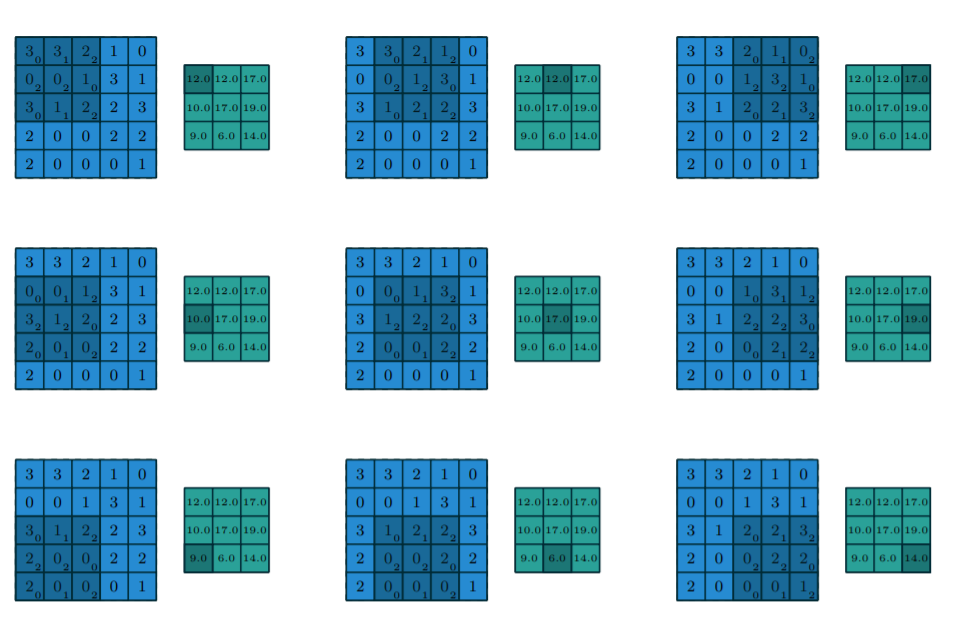
\includegraphics[width=200pt]{images/cnn/convolution.png}
\caption{Fonctionnement de la couche de convolution sur un exemple simple. L'image est tirée de l'article de Dumoulin et al. \cite{dumoulin_guide_2018}.}
\label{convolution}
\end{figure}

On remarque alors que le résultat a une dimension plus petite que l'image d'origine : on a ici effectué ce que l'on appelle un \textbf{simple padding}. Cependant, on pourrait souhaiter que le résultat ait la même dimension : cela est rendu possible grâce au \textbf{same padding}. Pour cela, nous pouvons rajouter des gardes autour de l'image d'origine : on rajoute des zéros autour puis on effectue l'opération de convolution comme présentée sur la figure \ref{same_padding}

\begin{figure}[!h]
\centering
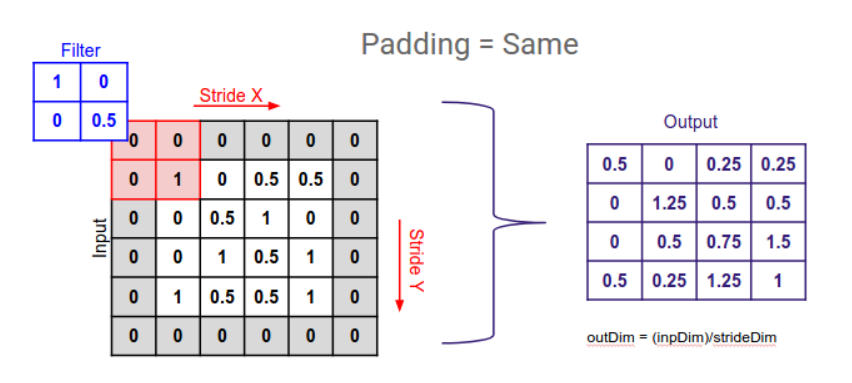
\includegraphics[width=200pt]{images/cnn/same_padding.png}
\caption{Fonctionnement de la couche de convolution avec du same padding. L'image est tirée de l'article de Dumoulin et al. \cite{dumoulin_guide_2018}.}
\label{same_padding}
\end{figure}

Il existe encore un paramètre permettant de personnaliser l'opération : le \textbf{stride}. Celui correspond au décalage à utiliser pour le noyau. Ce processus est représenté sur la figure \ref{stride}.

\begin{figure}[!h]
\centering
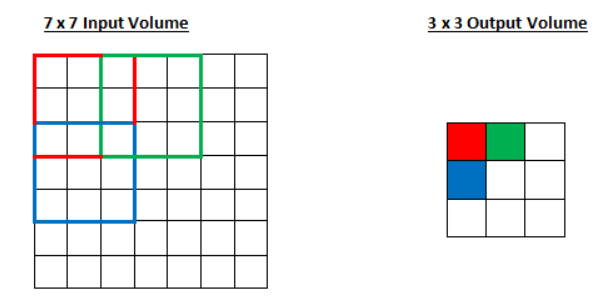
\includegraphics[width=150pt]{images/cnn/stride.png}
\caption{Fonctionnement de la couche de convolution avec un stride valant 2. À gauche, le résultat de l'opération. À droite, une façon différente de voir les choses : le noyau balaye toute la matrice avec un pas de 1 mais ne garde les valeurs que pour les déplacements pairs. L'image est tirée de l'article de Dumoulin et al. \cite{dumoulin_guide_2018}.}
\label{stride}
\end{figure}
 
L'avantage d'avoir un stride plus grand que 1 est aussi son désavantage : en effet il va permettre d'avoir un résultat en sortie de plus petite dimension mais en contrepartie, il provoque une perte d'information.

\subsection{Généralisation en 3D}

Les images en couleurs peuvent être représentées par une matrice 3D de profondeur 3. Pour pouvoir gérer ce cas, nous prenons des noyaux de la même profondeur que l'image, puis nous appliquons séparément le produit de convolution sur les profondeurs correspondantes, le résultat final n'étant que la somme des résultats sur chaque profondeur. Un exemple d'une telle opération est représenté par la figure \ref{CNN_3D}.

\begin{figure}[!h]
\centering
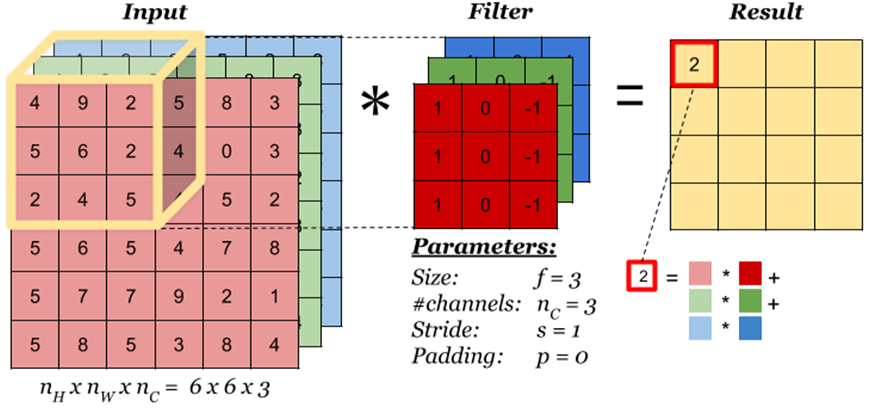
\includegraphics[width=150pt]{images/cnn/CNN_3D.png}
\caption{Exemple de convolution en 3D. L'image est tirée de l'article \textit{1D and 3D Convolution} de S.Verma \cite{verma_understanding_2020}.}
\label{CNN_3D}
\end{figure}

Notons cependant que ce résultat est très important car même si l'on considère que l'image n'a qu'une seule profondeur (image en niveau de gris par exemple), les données en entrée sur les autres couches de convolution sont dans l'immense majorité des cas en 3 dimensions. De manière intuitive, il est important de comprendre que la généralisation en 3D permet de détecter des motifs tridimensionnels au même titre qu'une opération de convolution simple permet d'identifier la présence d'un motif bidimensionnel. 

\subsection{Couche de pooling}

Les couches de pooling permettent de réduire la taille de la sortie au prix d'une perte d'information. Elles sont nécessaires pour compresser l'information. On considère généralement deux types de couches de pooling :

\begin{itemize}
 \item max pooling : on applique l'équivalent d'un noyau d'une opération de convolution qui ne retient que la valeur maximale de la zone sur laquelle il effectue les calculs. C'est la couche de pooling la plus utilisée. Un exemple de fonctionnement est présenté par la figure \ref{max_pooling}.
 
\begin{figure}[!h]
\centering
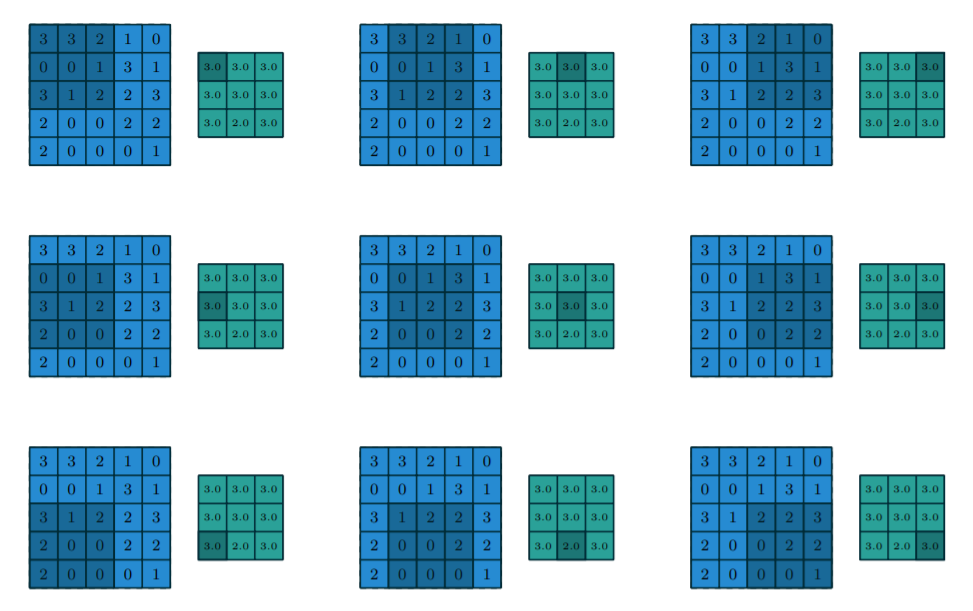
\includegraphics[width=200pt]{images/cnn/max_pooling.png}
\caption{Exemple simple d'application de la couche max pooling. L'image est tirée de l'article de Dumoulin et al. \cite{dumoulin_guide_2018}.}
\label{max_pooling}
\end{figure}
 
\item average pooling : le fonctionnement est le même que la couche de max pooling à sauf que l'on applique la fonction moyenne au lieu de la fonction maximum. Un exemple de fonctionnement est présenté par la figure \ref{avg_pooling}.
\end{itemize}

\begin{figure}[!h]
\centering
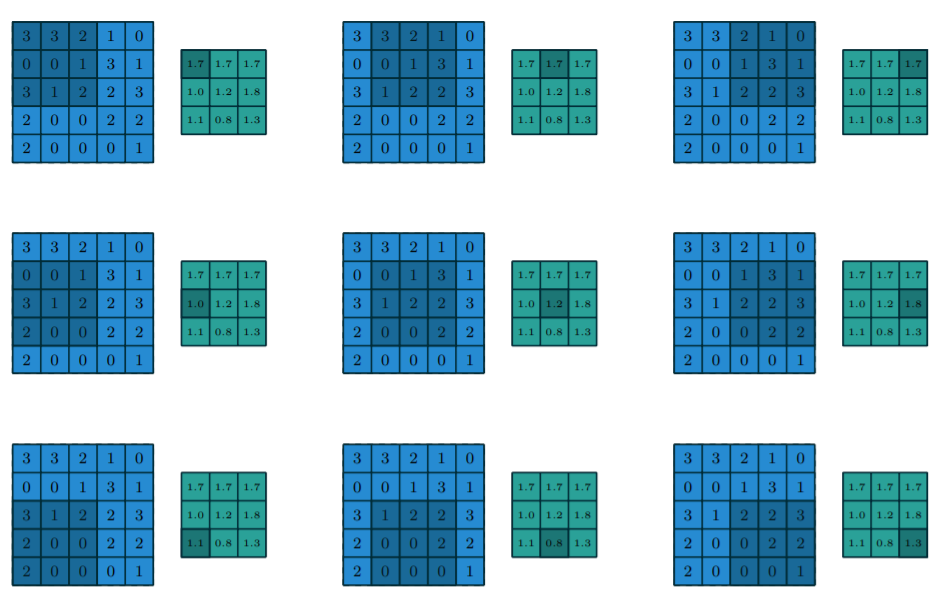
\includegraphics[width=200pt]{images/cnn/avg_pooling.png}
\caption{Exemple simple d'application de la couche avg pooling. L'image est tirée de l'article de Dumoulin et al. \cite{dumoulin_guide_2018}.}
\label{avg_pooling}
\end{figure}


Il est à noter que la taille des noyaux est une variable et que plus celle-ci est grande, plus la taille de la sortie sera petite. 
\subsection{Structure complète d'un CNN}

La reconnaissance d'objet est le plus souvent complexe et nécessite de nombreux motifs à déceler pour pouvoir être efficace. Ainsi, si l'on avait un motif par couche, la taille du CNN serait gigantesque. Pour éviter cela, il suffit d'associer à chaque couche plusieurs noyaux (généralement une puissance de 2). En appliquant les processus précédents pour chacun des noyaux, on se retrouve avec un nombre de matrice en sortie égal au nombre de noyaux. On se contente alors de les empiler en rajoutant une dimension supplémentaire. On obtient alors en sortie de couche de convolution, un bloc de profondeur égale au nombre de noyaux, contenant dans chacune des couches le résultat du produit de convolution pour un noyau. La figure \ref{structure_CNN_2} illustre ce principe.

\begin{figure}[!h]
\centering
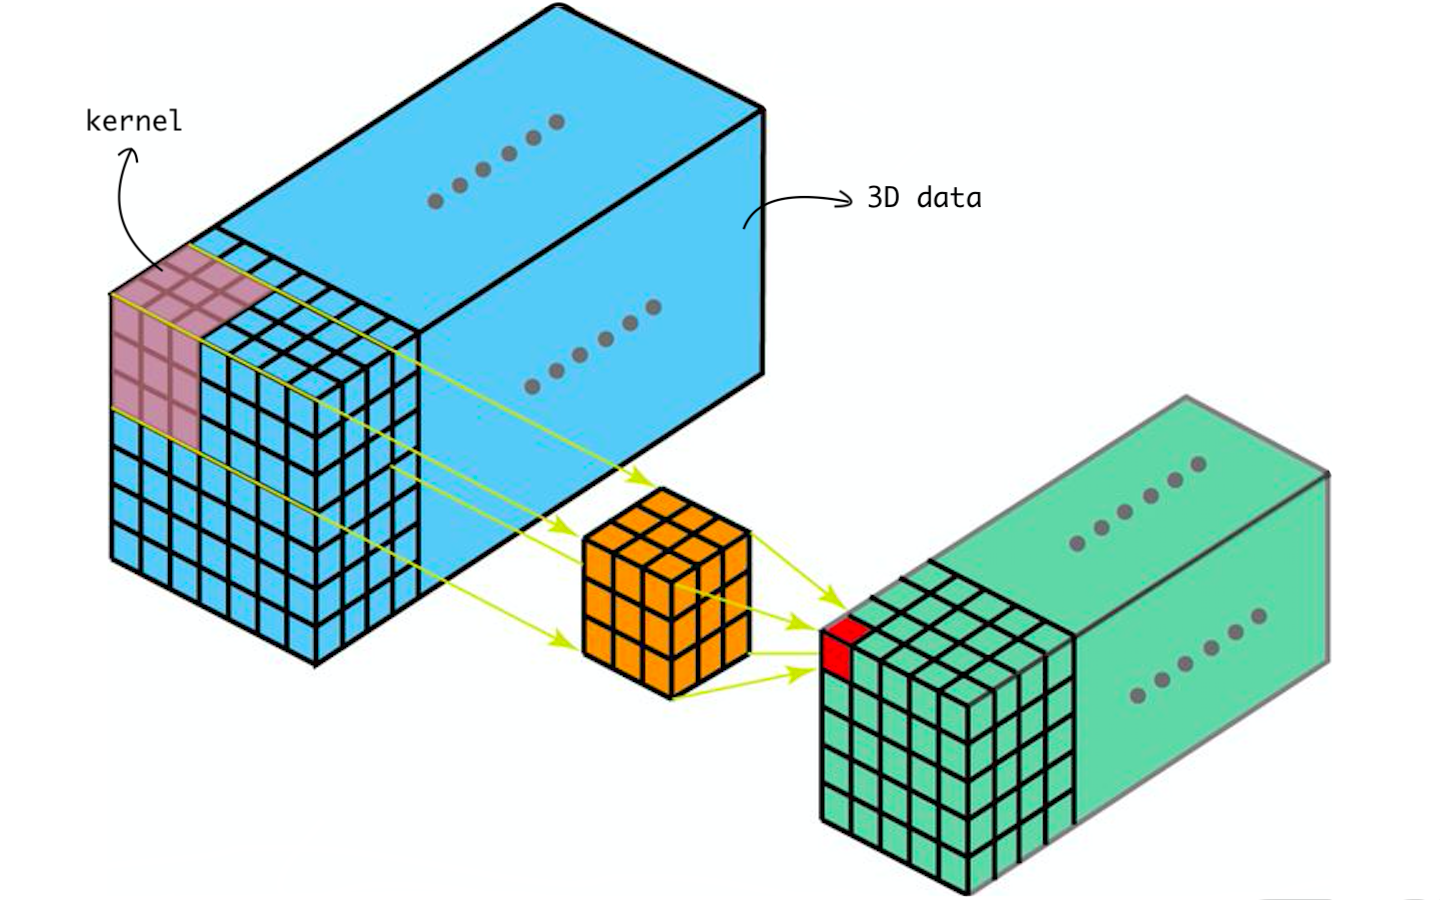
\includegraphics[width=200pt]{images/cnn/structure_CNN_2.png}
\caption{Exemple du résultat à la sortie d'une couche de convolution d'un CNN avec une structure complète. L'image est tirée de l'article \textit{1D and 3D Convolution} de S.Verma \cite{verma_understanding_2020}.}
\label{structure_CNN_2}
\end{figure}

On alterne ainsi entre couches de convolution pour prélever des motifs de plus en plus complexes et couches de pooling pour compresser les données. Les données étant ainsi pré-traitées, il suffit de les mettre en entrée d'une couche dense pour finalement avoir le résultat escompté.

\subsection{Apprentissage d'un CNN}

Le CNN, de par sa structure analogue à celle d'un MLP, a besoin d'une phase d'apprentissage dans le but d'apprendre à reconnaitre les motifs intéressants. Cela se fait par un processus de backpropagation. Cette partie étant essentiellement calculatoire, nous ne présenterons pas les opérations exactes à effectuer dans cette section. Les calculs sont essentiellement une généralisation de la rétropropagation présenté au chapitre 1. Pour plus d'informations, nous invitons le lecteur à consulter la littérature scientifique à ce sujet.
 
\subsection{Dropout}

Le principal problème de ce type d'architecture est le phénomène de sur-apprentissage. Pour pallier ce problème, des améliorations ont été proposées, notamment en 2014 par Srivastava et al. \cite{srivastava_dropout_nodate}. Les auteurs proposent en effet d'éteindre de manière aléatoire une certaine proportion de neurones (qui est un hyper-paramètre du dropout) pendant la phase de propagation avant (\textit{forward propagation}). Ils ont nommé cette technique le \textbf{dropout}. Cela permet de réduire la co-adaptation entre les neurones, évitant ainsi qu'un neurone ne prenne trop d'importance dans le processus d'apprentissage, ce qui pourrait amener à du sur-apprentissage. Une explication visuelle est proposée par la figure \ref{dropout}.

\begin{figure}[!h]
\centering
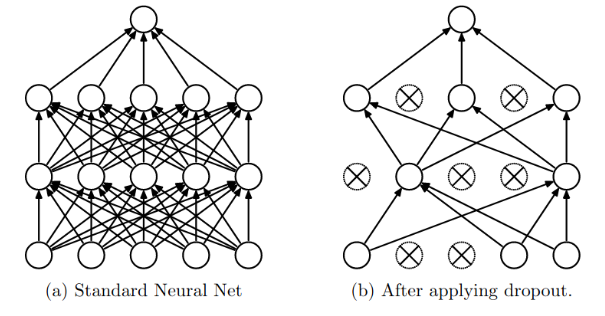
\includegraphics[width=200pt]{images/cnn/dropout.png}
\caption{A gauche, une structure MLP classique. A droite, un exemple de l'effet du dropout(paramètre ajusté à 50\%). Cette image vient de l'article de Srivastava et al. \cite{srivastava_dropout_nodate}.}
\label{dropout}
\end{figure}

La figure \ref{dropout_article} présente les résultats de ce même article. Les résultats sont plus que positifs dans la mesure où la qualité prédictive du réseau est grandement améliorée par le dropout.

\begin{figure}[!h]
\centering
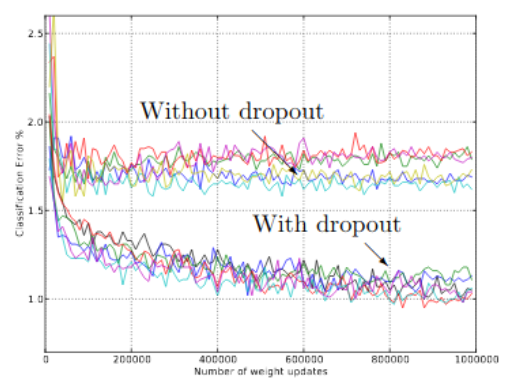
\includegraphics[width=200pt]{images/cnn/dropout_article.png}
\caption{Résultats de l'article sur l'efficacité du dropout sur un réseau neuronal. Cette image vient de l'article de Srivastava et al. \cite{srivastava_dropout_nodate}.}
\label{dropout_article}
\end{figure}
 
\section{Implémentation et résultats}

\subsection{Implémentation}

Nous avons une nouvelle fois utilisé TensorFlow 2.0 qui permet l'utilisation rapide de couches telles que celles de convolution, de pooling mais aussi de \textit{flatenning}. La couche de \textit{flatenning} est une couche permettant de faire la transition entre la dernière couche de convolution et la première couche dense. En d'autres termes, elle transforme les données en 3 dimensions en un tableau en 1 dimension.\\
La structure du réseau simplifié avec lequel nous avons fait les tests est la suivante :

\[ \begin{array}{lcr}
	Conv2D(64, 3, activation=relu) \\
    Conv2D(32, 3, activation=relu) \\
    Flatten() \\
    Dense(128, activation=relu) \\
    Dense(10, activation=softmax)\end{array}\]

Nous avons de plus utilisé l'optimiseur ADAM pour effectuer la descente de gradient.

\subsection{Résultats}

Nous avons tout d'abord voulu tester la taille des noyaux pour voir quelle influence celle-ci a sur les performances de notre CNN. La figure \ref{resultat_noyaux} présente les résultats sur la base de données MNIST.

\begin{figure}[!h]
\centering
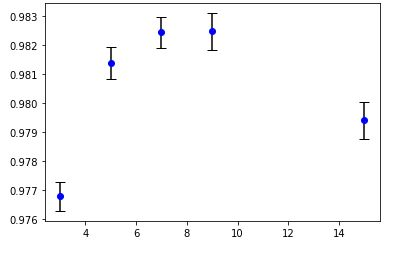
\includegraphics[width=150pt]{images/cnn/resultat_noyau.png}
\caption{Comparaison de la précision de notre CNN en fonction de la taille des noyaux. En ordonnée la précision, en abscisse la taille des noyaux. La base de données utilisée est MNIST.}
\label{resultat_noyaux}
\end{figure}

Nous pouvons en déduire que des noyaux de taille trop grande par rapport aux images d'origine risquent de nuire à l'efficacité du CNN. \\

Nous nous sommes, de plus, intéressés à l'influence du \textbf{stride} et du \textbf{padding} sur les performances du CNN. La figure \ref{resultat_padding_stride} présente les résultats de notre analyse sur MNIST.

\begin{figure}[!h]
\centering
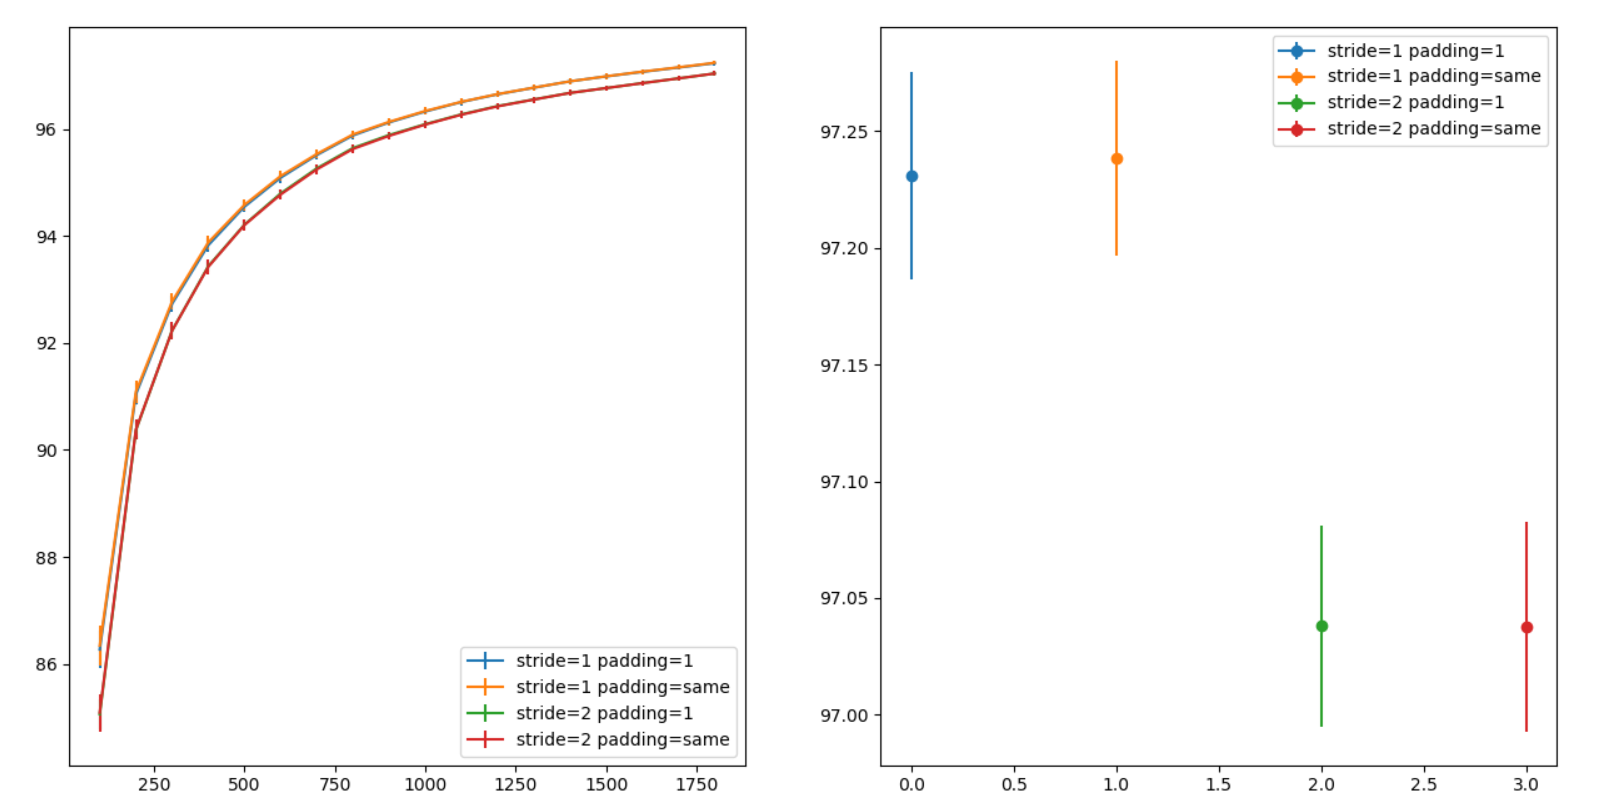
\includegraphics[width=230pt]{images/cnn/CNN_padding_stride.png}
\caption{Comparaison de la précision de notre CNN en fonction des paramètres stride et padding. En ordonnée la précision, en abscisse le nombre de batchs d’entraînement. La base de données utilisée est MNIST.}
\label{resultat_padding_stride}
\end{figure}

Nous pouvons conclure que, sur cette base de données, l'utilisation d'un stride supérieur à 1 a comme effet de réduire les capacités prédictives du CNN. En effet, lorsque ce paramètre est trop élevé, la perte d'information est trop importante, nuisant aux performances de l'algorithme. Nous remarquons de plus que le padding n'a ici aucune influence. Ce résultat n'est pas surprenant car les images de MNIST sont centrées avec des bords sombres. Ainsi il n'y a aucune information sur les bords, rendant le changement de padding quasiment inutile. \\

De même, nous avons testé l'influence du \textbf{dropout}. Les résultats sont présentés sur la figure \ref{resultat_dropout}. Les résultats sont beaucoup moins significatifs que ce que laisse présager l'article de Srivastava et al. \cite{srivastava_dropout_nodate}. Il semble donc que le dropout n'a aucune influence sur les résultats de notre CNN. Ceci est probablement dû à la banque d'images MNIST et à la petite taille de notre réseau, qui ne sont pas propices au sur-apprentissage .
  
\begin{figure}[!ht]
\centering
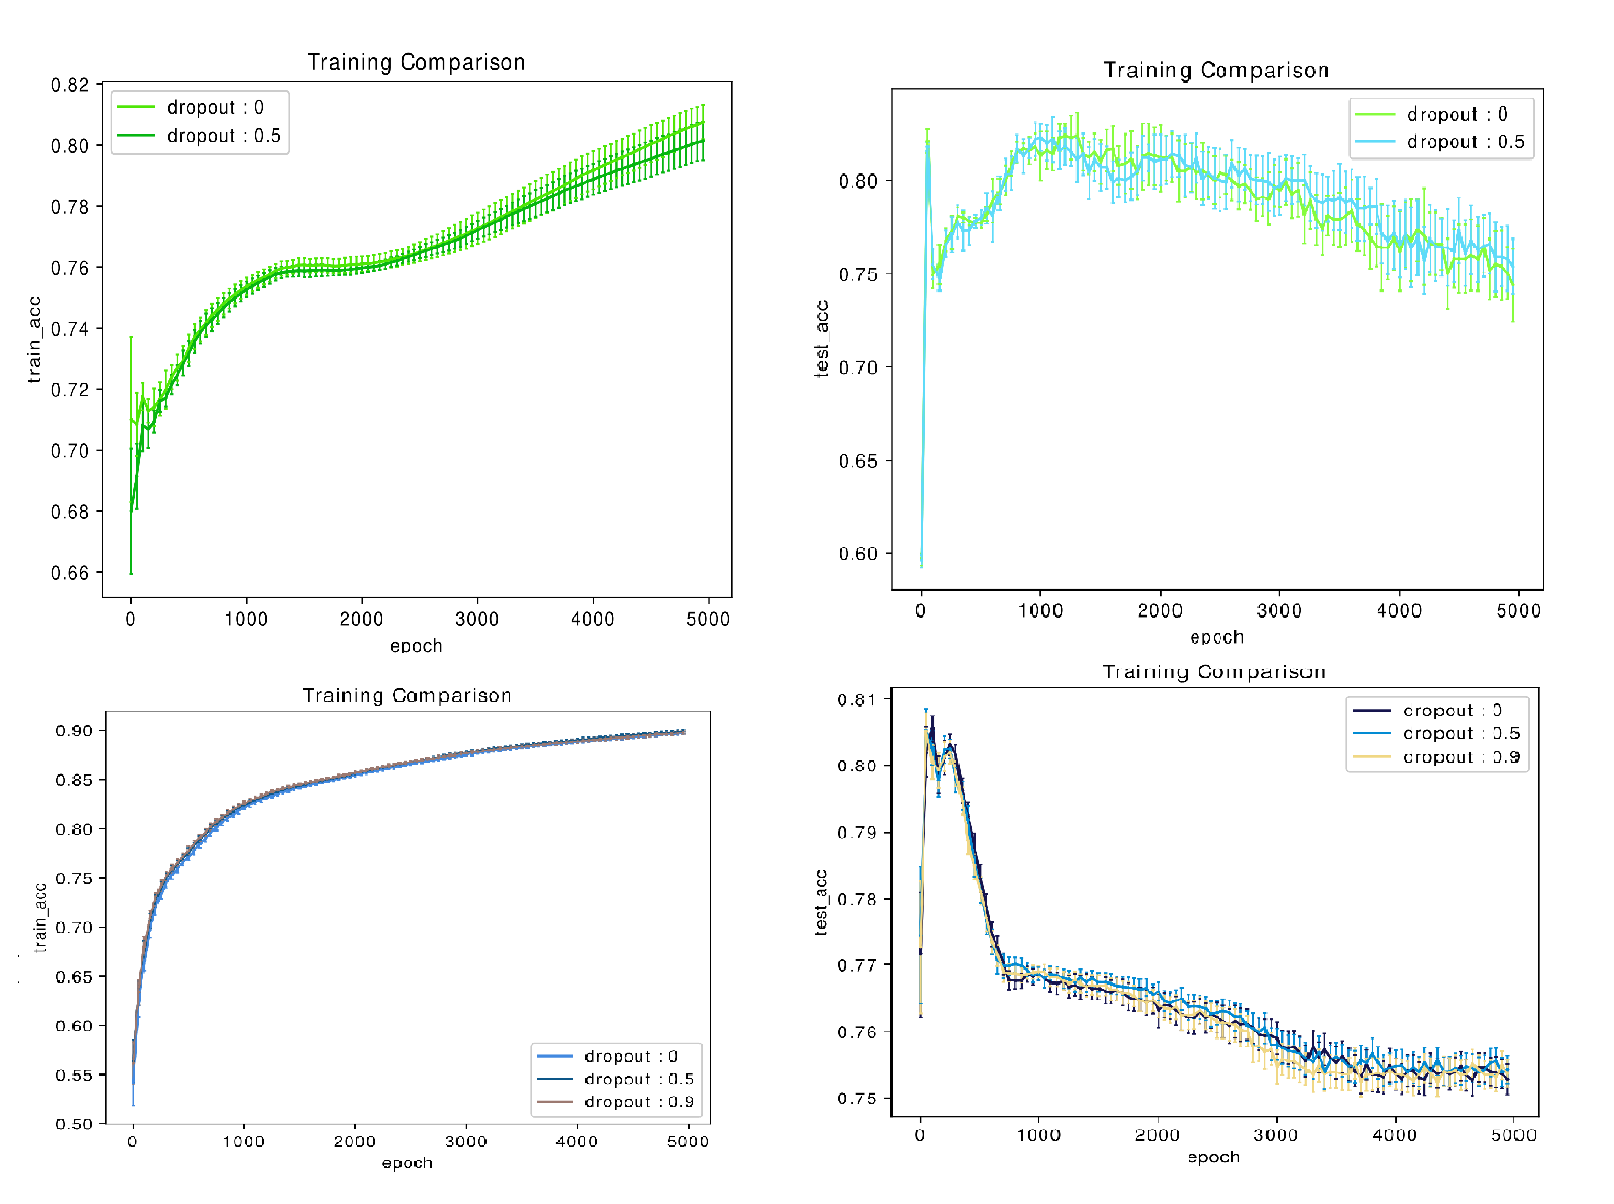
\includegraphics[width=260pt]{images/cnn/resultat_dropout.png}
\caption{Influence du dropout sur l'efficacité de nos réseaux. En haut, un CNN sur la base de données MNIST. En bas, un MLP sur la base de données Moon. Nous remarquons que les courbes sont toutes confondues, quel que soit le paramètre de dropout choisi.}
\label{resultat_dropout}
\end{figure}

 


